\section{Source, Ensemble, and Diagnostic Controls}\label{sec:controls}

\subsection{Fused and component supervision}
\label{sec:source-ablation}
Holding J fixed, mean gains are $+0.155665$ for F, $+0.134868$ for T, and $+0.040991$ for G. F exceeds T by $+0.020797\pm0.001214$ and G by $+0.114674\pm0.001001$, with both contrasts positive in all three seeds. Composition and predictive quality change together, so this does not isolate the source of fusion benefits.

The T-only eligibility gate and first formal epoch clip every update despite finite parameter gradients. The authorized continuation retains \texttt{CLIP\_SATURATION\_WARNING}. Interpret the modest F--T gap cautiously; Appendix~\ref{app:protocols} records the unchanged training protocol and clipping trajectory.

\subsection{Homogeneous ensemble falsification}
\label{sec:homogeneous-control}
TT gives gain $+0.168125\pm0.008948$ versus $+0.155665\pm0.007692$ for TG. The paired contrast is
\begin{equation}
H=\mathrm{Gain}_{\mathrm{TG}}-\mathrm{Gain}_{\mathrm{TT}}
=\mathrm{NLL}_{\mathrm{TT}}-\mathrm{NLL}_{\mathrm{TG}},
\label{eq:ensemble-contrast}
\end{equation}
with mean $-0.012460\pm0.001348$ and all three differences negative. The tested TG teacher provides no advantage over TT (Figure~\ref{fig:ensemble_control}).

TT also has a 0.010108 full-validation teacher-NLL advantage, approximately 6.38\% fewer parameters, and different fusion-learning-rate and training histories. These confounds prevent attributing the ordering to intrinsic TT superiority. TG has greater branch disagreement, but not greater KD gain; predictive diversity is not necessarily transferable diversity. This comparison does not support a Grassmann-specific or heterogeneous-supervision advantage.

\subsection{Local diagnostics do not separate endpoints}
\label{sec:local-diagnostics}
Across seven teacher--domain families and three student seeds per family, retrospective first- and second-order scores both achieve AUROC approximately 0.644 and sign accuracy approximately 0.571. Curvature adds no sign separation, and the scores misclassify known positive WikiText-2 families. The tested local diagnostics are not reliable predictors of these endpoints.

Some scalar predictors discriminate pooled outcomes better, but the small dependent collection does not establish a general selection rule. Token-level branch JSD adds little information beyond CE difficulty. Appendix~\ref{app:diagnostics-modern} reports full metrics, calibration instability, and observational limits. The failures concern the tested offline scores, not adaptive KD methods in general.

\begin{figure*}[!t]
\centering
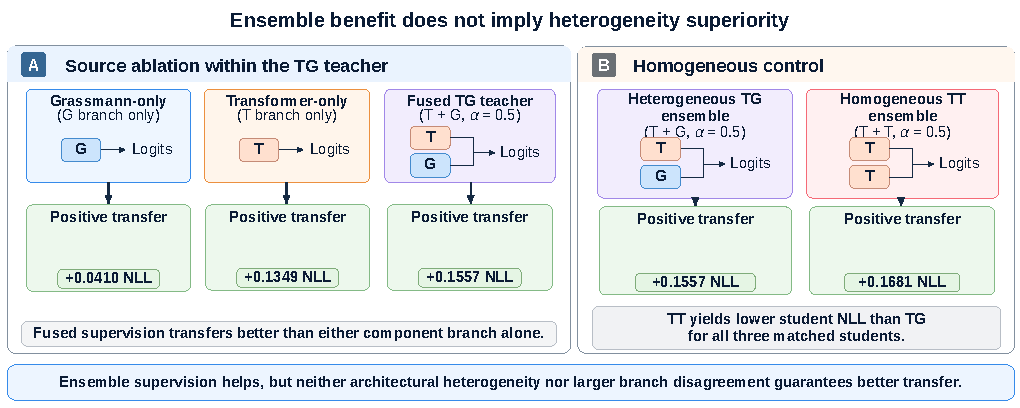
\includegraphics[width=\textwidth]{figures/fig4_ensemble_control.pdf}
\caption{WikiText-2 teacher-source and ensemble gains, rounded to four decimals. TT exceeds TG in all three students. T-only: early clipping saturation; interpret F--T gap cautiously. TT and TG teachers are not strictly quality- or training-matched.}
\label{fig:ensemble_control}
\end{figure*}
